\documentclass[letterpaper]{article} % DO NOT CHANGE THIS
\usepackage[submission]{aaai2027} % DO NOT CHANGE THIS

% Required by the official AAAI-27 template
\usepackage[hyphens]{url} % DO NOT CHANGE THIS
\usepackage{graphicx} % DO NOT CHANGE THIS
\urlstyle{rm} % DO NOT CHANGE THIS
\def\UrlFont{\rm} % DO NOT CHANGE THIS
\usepackage{natbib} % DO NOT CHANGE THIS AND DO NOT ADD OPTIONS
\usepackage{caption} % DO NOT CHANGE THIS AND DO NOT ADD OPTIONS
\frenchspacing % DO NOT CHANGE THIS

% Packages used by, or commonly needed by, this paper
\usepackage{amsmath}
\usepackage{amssymb}
\usepackage{booktabs}
\usepackage{multirow}

% Uncomment these two lines only if the paper contains algorithm environments.
% \usepackage{algorithm}
% \usepackage{algorithmic}

\pdfinfo{
/TemplateVersion (2027.1)
}

% The official template permits changing this to 1 or 2 if numbered
% section headings are desired.
\setcounter{secnumdepth}{0}

\title{ProtoDRIFT: Prototype-Disentangled Deviation-Referenced Invariant Forecasting for Transferable Cross-City Anomalous Urban Flows}

% Anonymous review version
\author{Anonymous Submission}
\affiliations{}

\begin{document}

\maketitle

\begin{abstract}
% 城市异常客流预测对于交通调度、公共安全和城市韧性管理具有重要意义，但异常样本稀疏且城市间分布不均，使得跨城市迁移预测仍然面临显著挑战。本文关注跨城市异常客流预测问题，即模型在源城市训练，并直接迁移到目标城市，在全量时段和异常时段上进行评估。我们提出 ProtoDRIFT，一个原型解耦的偏差参照不变预测框架。其核心思想是将城市客流分解为城市特定的正常基线和相对可迁移的异常偏差，并在偏差空间中学习可迁移异常原型，同时通过互信息约束解耦异常表示与城市特定表示。基于 NYC 与 CHI 的双向跨城市迁移实验将系统验证 ProtoDRIFT 在 full 与 anomaly 子集上的有效性，并通过消融、敏感性和可视化分析解释关键模块的作用。

Forecasting anomalous urban flows is critical for traffic scheduling, public safety, and urban resilience management. However, anomalous samples are scarce and unevenly distributed across cities, which makes cross-city transfer forecasting a significant challenge. This paper focuses on cross-city anomalous urban flow forecasting, where a model is trained on a source city and directly transferred to a target city for evaluation on both full and anomalous periods. We propose ProtoDRIFT, a prototype-disentangled, deviation-referenced invariant forecasting framework. Its core idea is to decompose urban flows into a city-specific normal baseline and relatively transferable anomaly deviations, learn transferable anomaly prototypes in the deviation space, and disentangle anomaly representations from city-specific representations via a mutual information constraint. Extensive bidirectional cross-city transfer experiments between NYC and CHI demonstrate the effectiveness of ProtoDRIFT on both the full and anomaly subsets, and ablation, sensitivity, and visualization analyses further explain the roles of its key modules.

\end{abstract}

\section{Introduction}

% 城市客流预测是智能交通系统中的基础任务之一，能够为交通调度、运力配置、拥堵缓解和公共安全管理提供关键支撑。随着城市传感器、交通卡口、共享出行和移动设备数据的持续积累，深度学习方法已经被广泛用于刻画客流序列中的时间周期性、空间相关性和长期动态变化。现有时空预测模型在常规通勤场景下取得了显著进展，但它们大多依赖相对稳定且充足的历史模式，默认未来客流会延续日周期、周周期或局部空间依赖等规律。因此，当城市运行状态偏离常规模式时，仅依靠常规历史模式进行预测往往难以满足实际需求。

Urban flow forecasting is one of the fundamental tasks in intelligent transportation systems, providing essential support for traffic scheduling, capacity allocation, congestion mitigation, and public safety management. With the continuous accumulation of data from urban sensors, traffic checkpoints, shared mobility, and mobile devices, deep learning methods have been widely adopted to characterize the temporal periodicity, spatial correlations, and long-term dynamics of flow sequences. Existing spatiotemporal forecasting models have achieved remarkable progress in regular commuting scenarios, but they largely rely on relatively stable and abundant historical patterns, implicitly assuming that future flows will follow daily/weekly periodicities and local spatial dependencies. Consequently, when the operating state of a city deviates from its regular patterns, forecasts that rely solely on regular historical patterns often fall short of practical requirements.

% 异常场景下的客流预测更加困难，也更具有现实意义。节假日、极端天气、大型活动和突发事件等因素会显著改变居民出行需求，使客流在时间强度、空间分布和变化趋势上都偏离正常通勤模式。针对这类问题，已有研究尝试引入事件信息、天气特征、鲁棒时序建模或异常增强的时空结构，以提升模型对稀有高影响时段的预测能力。这些方法在单城市异常预测中具有一定效果，但通常仍在绝对客流空间中直接建模，并且主要关注训练和测试分布相对一致的场景。由此带来的问题是，模型容易把城市本身的正常客流尺度、局部空间结构和异常造成的偏移混合在一起，难以区分哪些模式是城市特有的，哪些异常变化具有跨城市迁移价值。

Flow forecasting under anomalous scenarios is more difficult and of greater practical importance. Holidays, extreme weather, large-scale events, and emergencies can substantially reshape travel demand, driving flows away from normal commuting patterns in temporal intensity, spatial distribution, and evolving trends. To address such problems, prior studies have incorporated event information, weather features, robust temporal modeling, or anomaly-enhanced spatiotemporal structures to improve forecasting on rare but high-impact periods. These methods are effective for single-city anomaly forecasting to some extent, but they typically still model flows directly in the absolute-value space and mainly target scenarios where the training and test distributions are relatively consistent. As a consequence, models tend to entangle a city's inherent normal flow scale, local spatial structures, and anomaly-induced shifts, making it difficult to distinguish which patterns are city-specific and which anomalous variations are transferable across cities.

% 本文进一步关注一个更具体也更具挑战性的研究问题：跨城市异常客流预测，即模型在源城市上训练，并直接迁移到目标城市，在全量时段和异常时段上进行评估。这个问题具有实际价值，因为单个城市中的异常样本往往数量有限，而不同城市之间可能共享某些由节假日、天气或活动引发的异常变化规律。然而，直接进行跨城市迁移面临两个核心挑战。第一，异常客流样本稀疏，且与正常客流差异显著；模型在大量正常样本上训练时，容易低估异常偏移，或者将异常变化吸收到城市特定的正常基线中。第二，异常客流模式在不同城市之间分布不均，同类异常事件在发生频率、影响强度、空间覆盖范围和持续时间上都可能存在明显差异，因此在原始客流空间中直接迁移往往并不可靠。

This paper further focuses on a more specific and more challenging research problem: cross-city anomalous urban flow forecasting, where a model is trained on a source city and directly transferred to a target city for evaluation on both full and anomalous periods. This problem is of practical value because anomalous samples within a single city are often limited, whereas different cities may share certain anomalous variation patterns induced by holidays, weather, or events. However, direct cross-city transfer faces two core challenges. First, anomalous flow samples are scarce and differ markedly from normal flows; when trained on abundant normal samples, a model tends to underestimate anomalous shifts or absorb anomalous variations into the city-specific normal baseline. Second, anomalous flow patterns are unevenly distributed across cities; the same type of anomalous event may differ substantially in frequency, impact intensity, spatial coverage, and duration, so direct transfer in the raw flow space is often unreliable.

% 我们的核心观察是，城市客流可以被分解为城市特定的正常基线和相对更可迁移的异常偏差。相比直接迁移不同城市之间尺度差异显著的绝对客流值，我们首先利用正常基线刻画目标城市自身的常规出行模式，再在相对于该基线的偏差空间中学习异常动态。基于这一思想，本文提出 **ProtoDRIFT**，一个面向跨城市异常客流预测的原型解耦偏差参照不变预测框架。ProtoDRIFT 包含两个关键设计：其一是可迁移异常原型机制，通过紧凑的原型库归纳偏差空间中反复出现的异常变化模式，从而捕获较少依赖具体城市尺度的异常语义；其二是互信息约束的解耦设计，通过约束异常表示与城市特定表示之间的冗余依赖，促使模型区分可迁移异常偏差和本地城市因素。二者结合后，模型能够以目标城市正常基线为参照，叠加迁移得到并经过城市条件调整的异常偏差，从而完成目标城市客流预测。

Our key observation is that urban flows can be decomposed into a city-specific normal baseline and relatively more transferable anomaly deviations. Instead of directly transferring absolute flow values whose scales differ substantially across cities, we first characterize the target city's own regular travel patterns with a normal baseline, and then learn anomalous dynamics in the deviation space relative to this baseline. Based on this idea, we propose **ProtoDRIFT**, a prototype-disentangled, deviation-referenced invariant forecasting framework for cross-city anomalous urban flow forecasting. ProtoDRIFT features two key designs. The first is a \textbf{transferable anomaly prototype mechanism}, which summarizes recurring anomalous variation patterns in the deviation space with a compact prototype bank, thereby capturing anomaly semantics that are less dependent on city-specific scales. The second is a \textbf{mutual-information-constrained disentanglement design}, which restrains the redundant dependence between anomaly representations and city-specific representations, encouraging the model to distinguish transferable anomaly deviations from local city factors. Combining the two, the model produces target-city flow forecasts by taking the target city's normal baseline as a reference and superimposing the transferred, city-conditionally adjusted anomaly deviations.


% 本文的主要贡献包括三点。第一，我们将跨城市异常客流预测建模为一个偏差参照的迁移问题，提出“城市特定正常基线 + 可迁移异常偏差”的预测视角，以缓解绝对客流空间中城市尺度差异带来的迁移困难。第二，我们设计了 ProtoDRIFT 框架，通过可迁移异常原型和互信息约束的解耦机制，对稀疏异常样本中的共享偏差模式进行结构化建模。第三，我们在 NYC 与 CHI 的双向跨城市迁移设置下进行了系统实验，覆盖 `NYC→CHI` 和 `CHI→NYC` 两个 setting，并同时评估 full 与 anomaly 子集，通过主实验、消融实验、参数敏感性和可视化分析验证所提出设计的有效性。


Our main contributions are threefold.

\begin{itemize}
    \item \textbf{Conceptual insight.} We formulate cross-city anomalous urban flow forecasting as a deviation-referenced transfer problem and propose the forecasting perspective of "city-specific normal baseline + transferable anomaly deviation" to alleviate the transfer difficulty caused by city-scale discrepancies in the absolute flow space.
    \item \textbf{Methodological framework.} We design the ProtoDRIFT framework, which structurally models the shared deviation patterns in sparse anomalous samples via transferable anomaly prototypes and a mutual-information-constrained disentanglement mechanism. 
    \item \textbf{Empirical validation.} we conduct systematic experiments under the bidirectional cross-city transfer setting between NYC and CHI, covering both `NYC$\rightarrow$CHI` and `CHI$\rightarrow$NYC` settings and evaluating both the full and anomaly subsets, and validate the effectiveness of the proposed designs through main results, ablation studies, hyperparameter sensitivity, and visualization analyses.
\end{itemize}
\section{Preliminaries}

\textbf{Definition 1 (Urban Flow Observations).} For each city $c$ in a set $\mathcal{C}$ with $N_c$ spatial units, we observe a flow sequence $\mathbf{X}^{(c)}=[\mathbf{x}^{(c)}_1,\ldots,\mathbf{x}^{(c)}_{T_c}]\in\mathbb{R}^{T_c\times N_c}$. A forecasting sample $(\mathbf{X}^{(c)}_{t-H+1:t},\mathbf{Y}^{(c)}_{t+1:t+P})$ uses $H$ historical steps to predict the next $P$ steps, with $\mathbf{Y}^{(c)}_{t+1:t+P}=\mathbf{X}^{(c)}_{t+1:t+P}$.

\noindent\textbf{Definition 2 (Anomalous Flow Context).} Let $\mathbf{m}^{(c)}\in\{0,1\}^{T_c}$ be the anomaly context sequence, where $m^{(c)}_t=1$ marks a step affected by holidays, extreme weather, or other external disturbances. The future-window anomaly indicator is
\begin{equation}
    a^{(c)}_t=\mathbb{I}\left(\sum_{\tau=t+1}^{t+P}m^{(c)}_\tau>0\right).
\end{equation}
Samples with $a^{(c)}_t=1$ form the anomaly subset; all samples form the full subset.

\noindent\textbf{Problem Formulation (Cross-City Anomalous Urban Flow Forecasting).} Given a source city $c_s$ and a target city $c_t$ ($c_s\neq c_t$) that differ in node number, flow scale, periodicity, and anomaly distribution, we train on source samples $\mathcal{D}_s$ and directly apply the model to target test samples $\mathcal{D}_t$:
\begin{equation}
\begin{gathered}
    \theta^*=\arg\min_\theta\sum_{t\in\mathcal{T}_s}\ell\left(f_\theta(\mathbf{X}^{(c_s)}_{t-H+1:t}),\mathbf{Y}^{(c_s)}_{t+1:t+P}\right),\\
    \widehat{\mathbf{Y}}^{(c_t)}_{t+1:t+P}=f_{\theta^*}(\mathbf{X}^{(c_t)}_{t-H+1:t}).
\end{gathered}
\end{equation}
The key challenge is transferring forecasting knowledge to target-city anomalous periods under coexisting cross-city distribution shift and anomaly scarcity.
\section{Methodology}

% ProtoDRIFT 的核心思想是将跨城市异常客流预测从原始客流空间转化到相对于城市正常状态的偏差空间中进行建模。对于任意城市 $c$，原始客流 $\mathbf{X}^{(c)}$ 同时包含城市自身的长期通勤规律、空间规模差异以及异常事件造成的短期扰动。如果直接在 $\mathbf{X}^{(c)}$ 上学习跨城市预测函数，模型容易把城市特定的常规模式误认为可迁移异常模式。为此，ProtoDRIFT 首先为每个城市构造正常参照，再学习相对于该参照的异常偏差，并通过原型学习和互信息约束解耦分别刻画可迁移异常语义与城市条件差异。
% 整体而言，ProtoDRIFT 包含四个主要步骤。首先，根据非异常历史观测构造城市特定的正常参照 $\mathbf{B}^{(c)}$，并将输入客流转换为偏差表示 $\boldsymbol{\Delta}^{(c)}$。其次，在偏差空间中学习一组可迁移异常原型，用于归纳不同城市间共享的异常变化模式。再次，通过互信息约束的双分支结构分离异常类型表示和城市条件表示，避免共享异常语义被城市特定因素污染。最后，模型将未来正常参照、可迁移异常原型预测项和城市条件调整项组合起来，得到目标城市未来客流预测：

The core idea of ProtoDRIFT is to reformulate cross-city anomalous urban flow forecasting from the raw flow space into a deviation space relative to each city's normal state. For any city $c$, the raw flows $\mathbf{X}^{(c)}$ simultaneously contain the city's long-term commuting regularities, spatial-scale differences, and short-term disturbances caused by anomalous events. If a cross-city forecasting function is learned directly on $\mathbf{X}^{(c)}$, the model is prone to mistaking city-specific regular patterns for transferable anomalous patterns. To this end, ProtoDRIFT first constructs a normal reference for each city, then learns anomaly deviations relative to this reference, and characterizes transferable anomaly semantics and city-conditioned differences separately through prototype learning and mutual-information-constrained disentanglement.

Overall, ProtoDRIFT consists of four main steps. First, it constructs a city-specific normal reference $\mathbf{B}^{(c)}$ from non-anomalous historical observations and converts the input flows into deviation representations $\boldsymbol{\Delta}^{(c)}$. Second, it learns a set of transferable anomaly prototypes in the deviation space to summarize anomalous variation patterns shared across cities. Third, it separates the anomaly-type representation from the city-conditioned representation through a mutual-information-constrained dual-branch structure, preventing the shared anomaly semantics from being contaminated by city-specific factors. Finally, the model combines the future normal reference, the transferable prototype-based deviation term, and the city-conditioned adjustment term to produce the target flow forecast:

\begin{equation}
    \begin{aligned}
        \widehat{\mathbf{Y}}^{(c)}_{t+1:t+P} = \mathbf{B}^{(c)}_{t+1:t+P} + \widehat{\boldsymbol{\Delta}}^{(c)}_{\mathrm{type}} + \widehat{\boldsymbol{\Delta}}^{(c)}_{\mathrm{adj}},
    \end{aligned}
\end{equation}

\subsection{Transferable Anomaly Prototype Design}

% 跨城市异常预测的首要困难在于，不同城市的绝对客流规模和常规周期模式差异显著，而异常事件引发的相对变化可能具有更强的共享语义。因此，ProtoDRIFT 不直接在原始客流空间中学习异常模式，而是先构造城市特定的正常参照，再在偏差空间中进行原型建模。
% 给定城市 $c$ 的历史观测，正常参照函数 $\mathcal{B}^{(c)}(\cdot)$ 用于估计非异常上下文下的常规客流状态。对输入窗口和预测窗口，分别记：在实现上，$\mathcal{B}^{(c)}$ 可以由非异常历史观测统计得到，例如按空间单元、星期属性和小时属性聚合常规客流模式。该参照不承担最终预测功能，而是用于从原始客流中剥离城市特定的正常成分。输入窗口的偏差表示定义为：
% 为了进一步减弱不同城市间客流幅度差异，ProtoDRIFT 对偏差进行尺度归一化：
% 其中 $\sigma^{(c)}_{\Delta}$ 表示城市 $c$ 的偏差尺度统计量，$\epsilon$ 为数值稳定项。随后，异常编码器 $\mathrm{AEnc}(\cdot)$ 将归一化偏差映射为异常表示：
% 为了获得紧凑且可迁移的异常模式表达，ProtoDRIFT 引入异常原型库 $\mathcal{P}={(\mathbf{e}_k,\mathbf{r}_k)}_{k=1}^{K}$，其中 $\mathbf{e}_k$ 是第 $k$ 个原型的嵌入，$\mathbf{r}_k$ 是对应的未来偏差模式。给定异常表示 $\mathbf{z}_a$，模型根据其与各原型嵌入的距离计算原型分配权重：
% 由此，可迁移异常原型预测项表示为：
% 这一设计使模型不需要为每个城市记忆大量异常样本，而是通过有限数量的原型概括偏差空间中的典型异常形态。正常参照减少城市尺度干扰，偏差表示突出异常相对变化，原型库则为跨城市共享异常语义提供可解释的结构化载体。

The primary difficulty of cross-city anomaly forecasting is that the absolute flow scales and regular periodic patterns differ substantially across cities, whereas the relative variations induced by anomalous events may carry stronger shared semantics. Therefore, instead of learning anomalous patterns directly in the raw flow space, ProtoDRIFT first constructs a city-specific normal reference and then performs prototype modeling in the deviation space.

Given the historical observations of city $c$, the normal reference function $\mathcal{B}^{(c)}(\cdot)$ estimates the regular flow state under non-anomalous contexts. We denote input window as $\mathbf{B}^{(c)}_{t-H+1:t}$ and the prediction window $\mathbf{B}^{(c)}_{t+1:t+P}$. In practice, $\mathcal{B}^{(c)}$ can be estimated from non-anomalous historical observations, e.g., by aggregating regular flow patterns over spatial units, day-of-week, and hour-of-day attributes. This reference is not responsible for the final prediction itself; instead, it serves to strip the city-specific normal component from the raw flows. Therefore, the deviation representation of the input window is defined as $\boldsymbol{\Delta}^{(c)}_{t-H+1:t} = \mathbf{X}^{(c)}_{t-H+1:t} - \mathbf{B}^{(c)}_{t-H+1:t}.$

To further reduce the flow-magnitude discrepancies across cities, ProtoDRIFT applies scale normalization to the deviations $\widetilde{\boldsymbol{\Delta}}^{(c)}_{t-H+1:t} = \frac{\boldsymbol{\Delta}^{(c)}_{t-H+1:t}}{\sigma^{(c)}_{\Delta}}$, where $\sigma^{(c)}_{\Delta}$ is the deviation-scale statistic of city $c$. The anomaly encoder $\mathrm{AEnc}(\cdot)$ then maps the normalized deviations into the anomaly representation:

\begin{equation}
    \begin{aligned}
        \mathbf{z}_a = \mathrm{AEnc}\left(\widetilde{\boldsymbol{\Delta}}^{(c)}_{t-H+1:t}\right),
    \end{aligned}
\end{equation}

To obtain a compact and transferable expression of anomalous patterns, ProtoDRIFT introduces an anomaly prototype bank $\mathcal{P}={(\mathbf{e}_k,\mathbf{r}_k)}_{k=1}^{K}$, where $\mathbf{e}_k$ is the embedding of the $k$-th prototype and $\mathbf{r}_k$ is its associated future deviation pattern. Given the anomaly representation $\mathbf{z}_a$, the model computes the prototype assignment weights according to its distances to the prototype embeddings:
\begin{equation}
    \begin{aligned}
        w_k = \frac{\exp\left(-d(\mathbf{z}_a,\mathbf{e}_k)\right)}{\sum_{j=1}^{K}\exp\left(-d(\mathbf{z}_a,\mathbf{e}_j)\right)},
    \end{aligned}
\end{equation}
The transferable prototype-based deviation term is then expressed as $\widehat{\boldsymbol{\Delta}}^{(c)}_{\mathrm{type}} = \sum_{k=1}^{K} w_k \mathbf{r}_k$. With this design, the model does not need to memorize a large number of anomalous samples for each city; instead, it summarizes the typical anomalous shapes in the deviation space with a limited number of prototypes. The normal reference reduces the interference of city scales, the deviation representation highlights the relative anomalous variations, and the prototype bank provides an interpretable, structured carrier for anomaly semantics shared across cities.


\subsection{Mutual-Information-Constrained Disentanglement}

% 仅依赖异常原型仍不足以完全解决跨城市迁移问题。即使在偏差空间中，异常变化也可能包含城市特定的响应幅度、局部空间结构和事件影响范围。如果这些因素被混入可迁移异常表示，模型在目标城市上仍可能出现迁移偏差。因此，ProtoDRIFT 进一步引入互信息约束的解耦设计，将异常类型表示与城市条件表示分开建模。
% 具体而言，模型使用异常分支从归一化偏差中提取可迁移异常表示 $\mathbf{z}_a$，同时使用城市条件分支从原始偏差中提取城市特定表示 $\mathbf{z}_s$：
% 其中，$\mathbf{z}_a$ 主要服务于异常原型匹配，刻画跨城市共享的异常类型；$\mathbf{z}_s$ 则保留与城市条件相关的局部偏差信息，用于生成城市特定调整项。给定 $\mathbf{z}_s$，城市调整解码器 $\mathrm{CAD}(\cdot)$ 输出：
% 为了避免 $\mathbf{z}_a$ 与 $\mathbf{z}_s$ 学到高度重叠的信息，ProtoDRIFT 对二者引入互信息约束：
% 其中 $\widehat{I}(\cdot;\cdot)$ 表示对两个表示之间互信息的可优化估计。训练时最小化该项可以降低异常分支和城市条件分支之间的信息冗余，促使 $\mathbf{z}_a$ 更集中于异常类型，$\mathbf{z}_s$ 更集中于城市条件调整。需要强调的是，互信息约束并不单独等价于严格的城市不变性保证；它与偏差空间建模、尺度归一化和容量约束共同作用，形成更适合跨城市异常迁移的表示分工。

Anomaly prototypes alone are still insufficient to fully address cross-city transfer. Even in the deviation space, anomalous variations may contain city-specific response magnitudes, local spatial structures, and event coverage. If such factors leak into the transferable anomaly representation, the model may still suffer from transfer bias in the target city. ProtoDRIFT therefore further introduces a mutual-information-constrained disentanglement design that models the anomaly-type representation and the city-conditioned representation separately.

Specifically, the anomaly branch extracts the transferable anomaly representation $\mathbf{z}_a$ from the normalized deviations, while the city-conditioned branch extracts the city-specific representation $\mathbf{z}_s$ from the raw deviations:

\begin{equation}
\begin{gathered}
    \mathbf{z}_a = \mathrm{AEnc}\left(\widetilde{\boldsymbol{\Delta}}^{(c)}_{t-H+1:t}\right), \\
    \mathbf{z}_s = \mathrm{CEnc}\left(\boldsymbol{\Delta}^{(c)}_{t-H+1:t}\right),
\end{gathered}
\end{equation}
Here, $\mathbf{z}_a$ mainly serves prototype matching and characterizes the anomaly types shared across cities, whereas $\mathbf{z}_s$ preserves the local deviation information related to city conditions and is used to generate the city-specific adjustment term. Given $\mathbf{z}_s$, the city adjustment decoder $\mathrm{CAD}(\cdot)$ outputs $\widehat{\boldsymbol{\Delta}}^{(c)}_{\mathrm{adj}} = \mathrm{CAD}(\mathbf{z}_s)$. To prevent $\mathbf{z}_a$ and $\mathbf{z}_s$ from learning highly overlapping information, ProtoDRIFT imposes a mutual information constraint on the two representations:

\begin{equation}
    \begin{aligned}
        \mathcal{L}_{\mathrm{mic}} = \widehat{I}(\mathbf{z}_a;\mathbf{z}_s),
    \end{aligned}
\end{equation}
where $\widehat{I}(\cdot;\cdot)$ denotes an optimizable estimate of the mutual information between the two representations. Minimizing this term during training reduces the information redundancy between the anomaly branch and the city-conditioned branch, encouraging $\mathbf{z}_a$ to focus on anomaly types and $\mathbf{z}_s$ on city-conditioned adjustments. We emphasize that the mutual information constraint alone is not equivalent to a strict guarantee of city invariance; rather, it works in concert with deviation-space modeling, scale normalization, and the capacity constraint to form a division of representational labor that better suits cross-city anomaly transfer.


\subsection{Training Objective}

% ProtoDRIFT 的训练目标由预测损失和多个结构化正则项共同组成。首先，最终预测结果为未来正常参照、异常原型预测项和城市条件调整项之和：
% 预测损失约束模型输出接近真实未来客流：
% 除预测损失外，ProtoDRIFT 还引入容量约束、互信息约束、原型约束和调整约束，以稳定两个核心设计的学习过程。总体训练目标为：
% 其中，$\mathcal{L}_{\mathrm{cap}}$ 用于限制异常表示容量，减少城市特定细节泄漏到可迁移分支；$\mathcal{L}_{\mathrm{mic}}$ 降低异常表示与城市条件表示之间的冗余；$\mathcal{L}_{\mathrm{proto}}$ 提升异常原型的判别性和使用稳定性；$\mathcal{L}_{\mathrm{adj}}$ 约束城市调整分支，避免其完全覆盖共享异常原型的作用。通过这些目标的联合优化，模型既能保持最终预测精度，又能维持可迁移异常表示和城市条件表示之间的功能分工。

The training objective of ProtoDRIFT combines the forecasting loss with several structured regularization terms. First, the final prediction is the sum of the future normal reference, the prototype-based deviation term, and the city-conditioned adjustment term. The forecasting loss drives the model output toward the ground-truth future flows:

\begin{equation}
    \begin{aligned}
        \mathcal{L}_{\mathrm{pred}}
= \ell\left(\widehat{\mathbf{Y}}^{(c)}_{t+1:t+P},\mathbf{Y}^{(c)}_{t+1:t+P}\right),
    \end{aligned}
\end{equation}

Beyond the forecasting loss, ProtoDRIFT introduces a capacity constraint, a mutual information constraint, a prototype regularization, and an adjustment regularization to stabilize the learning of the two core designs. The overall training objective is:

\begin{equation}
    \begin{aligned}
        \mathcal{L} = \mathcal{L}_{\mathrm{pred}} + \alpha \mathcal{L}_{\mathrm{cap}} + \beta \mathcal{L}_{\mathrm{mic}} + \gamma \mathcal{L}_{\mathrm{proto}} + \zeta \mathcal{L}_{\mathrm{adj}},
    \end{aligned}
\end{equation}

Specifically, $\mathcal{L}_{\mathrm{cap}}$ limits the capacity of the anomaly representation to reduce the leakage of city-specific details into the transferable branch; $\mathcal{L}_{\mathrm{mic}}$ reduces the redundancy between the anomaly representation and the city-conditioned representation; $\mathcal{L}_{\mathrm{proto}}$ improves the discriminability and usage stability of the anomaly prototypes; and $\mathcal{L}_{\mathrm{adj}}$ regularizes the city adjustment branch so that it does not fully override the shared anomaly prototypes. Jointly optimizing these objectives allows the model to maintain forecasting accuracy while preserving the functional division between the transferable anomaly representation and the city-conditioned representation.



\subsection{Cross-City Inference}

% 在跨城市设置下，ProtoDRIFT 先在源城市 $c_s$ 上学习异常原型、解耦表示和预测目标，然后将训练后的主体参数迁移到目标城市 $c_t$。与依赖固定节点集合或城市专属图结构的方法不同，ProtoDRIFT 的推理过程不要求源城市与目标城市具有相同的空间单元数量，也不需要为目标城市重新设计节点嵌入或邻接结构。
% 给定目标城市输入窗口 $\mathbf{X}^{(c_t)}_{t-H+1:t}$，模型首先构造目标城市自身的正常参照 $\mathbf{B}^{(c_t)}$，并计算目标偏差表示：
% 随后，模型复用源城市训练得到的异常编码器、原型库、城市条件编码器和调整解码器，得到 $\widehat{\boldsymbol{\Delta}}^{(c_t)}_{\mathrm{type}}$ 与 $\widehat{\boldsymbol{\Delta}}^{(c_t)}_{\mathrm{adj}}$，并输出目标城市预测：
% 因此，ProtoDRIFT 的跨城市适配主要发生在目标城市正常参照和偏差表示构造阶段，而异常原型与解耦表示模块可以从源城市迁移使用。这种设计使模型能够在不同城市尺度和异常分布下复用共享异常语义，同时保留对目标城市局部客流响应的调整能力。

Under the cross-city setting, ProtoDRIFT first learns the anomaly prototypes, the disentangled representations, and the forecasting objective on the source city $c_s$, and then transfers the trained main parameters to the target city $c_t$. Unlike methods that rely on a fixed node set or city-specific graph structures, the inference procedure of ProtoDRIFT neither requires the source and target cities to share the same number of spatial units, nor needs re-designed node embeddings or adjacency structures for the target city.

Given the target-city input window $\mathbf{X}^{(c_t)}_{t-H+1:t}$, the model first constructs the target city's own normal reference $\mathbf{B}^{(c_t)}$ and computes the target deviation representation $\boldsymbol{\Delta}^{(c_t)}_{t-H+1:t} = \mathbf{X}^{(c_t)}_{t-H+1:t} - \mathbf{B}^{(c_t)}_{t-H+1:t}$. The model then reuses the anomaly encoder, the prototype bank, the city-conditioned encoder, and the adjustment decoder trained on the source city to obtain $\widehat{\boldsymbol{\Delta}}^{(c_t)}_{\mathrm{type}}$ and $\widehat{\boldsymbol{\Delta}}^{(c_t)}_{\mathrm{adj}}$, and outputs the target-city forecast:

\begin{equation}
    \begin{aligned}
        \widehat{\mathbf{Y}}^{(c_t)}_{t+1:t+P} = \mathbf{B}^{(c_t)}_{t+1:t+P} + \widehat{\boldsymbol{\Delta}}^{(c_t)}_{\mathrm{type}} + \widehat{\boldsymbol{\Delta}}^{(c_t)}_{\mathrm{adj}},
    \end{aligned}
\end{equation}

Therefore, the cross-city adaptation of ProtoDRIFT mainly takes place in the construction of the target city's normal reference and deviation representation, whereas the anomaly prototypes and the disentangled representation modules are transferred from the source city. This design enables the model to reuse shared anomaly semantics under different city scales and anomaly distributions, while retaining the ability to adjust to the target city's local flow responses.

\section{Experiment}

In this section, we conduct systematic experiments to answer the following four research questions:

\begin{itemize}
    \item RQ1: Under the bidirectional cross-city transfer setting, how does ProtoDRIFT perform on both full and anomalous periods compared with existing methods?
    \item RQ2: How much does each core module of ProtoDRIFT contribute to cross-city anomaly forecasting performance?
    \item RQ3: Is ProtoDRIFT sensitive to the values of its key hyperparameters?
    \item RQ4: Are the anomaly prototypes and disentangled representations learned by ProtoDRIFT interpretable?
\end{itemize}

\subsection{Experimental Setup}

\noindent \textbf{Datasets.} We conduct experiments on real-world taxi flow data from New York City (NYC) and Chicago (CHI), where NYC contains 820 spatial nodes and CHI contains 585 spatial nodes, spanning from 2014-10-01 to 2017-09-29 with a temporal granularity of 60 minutes. Both cities are split by calendar-aligned months into training (15336 steps), validation (5160 steps), and test (5784 steps) sets, and samples are constructed with a sliding window that predicts the future $P=12$ steps from the past $H=12$ steps. Anomalous periods are jointly annotated by holiday calendars and extreme weather records: a sample is assigned to the anomaly subset when the ratio of anomalous time steps within its prediction window is no less than 0.5. In the end, the NYC test set contains 5761 full samples (including 507 anomalous ones), and the CHI test set contains 5761 full samples (including 398 anomalous ones).

\noindent \textbf{Baselines.} We compare ProtoDRIFT with 11 representative methods in three categories: (1) conventional deep time series forecasting methods, including LSTM~\cite{lstm}, DLinear~\cite{dlinear}, PatchTST~\cite{PatchTST}, TimesNet~\cite{timesnet}, and ModernTCN~\cite{moderntcn}, which represent the mainstream paradigms
of single-city time series forecasting; (2) distributionally robust and transferable forecasting methods, including TimeAlign~\cite{timealign} and ProtoTS~\cite{protots}, which address distribution shifts via distribution alignment and hierarchical prototype learning, respectively; (3) anomaly/extreme-event-aware forecasting methods, including EVL~\cite{evl}, EALGAP~\cite{ealgap}, DAN~\cite{dan}, and ST-SSDL~\cite{stssdl}, which design dedicated losses or structures for extreme values and anomalous periods. All baselines adopt channel-independent modeling in our implementation, which supports zero-shot cross-city transfer between cities with different numbers of nodes.

\noindent \textbf{Implementation.} All methods share the same data splits, normalization pipeline, and evaluation scripts to ensure fairness: input data are normalized by a per-node StandardScaler and clipped to $[-10, 10]$, with statistics fitted only on the training set of each city. Training uses the Adam optimizer with a CosineAnnealingLR learning rate schedule and early stopping with a patience of 10. The default hyperparameters of ProtoDRIFT are $\alpha=0.3$, $K=8$, $\gamma=0.1$, and $\beta=0.01$ (see the sensitivity analysis in Section 4.4). We adopt MAE, RMSE, and $R^2$ as evaluation metrics, where lower MAE/RMSE is better and higher $R^2$ indicates a stronger ability to explain the flow variations of the target city; for each transfer direction, results are reported on both the full and anomaly test subsets.

\begin{table*}[htbp]
\centering
% \small
\setlength{\tabcolsep}{3.5pt}
\renewcommand\arraystretch{1.0}
\begin{tabular}{l|ccc|ccc|ccc|ccc}
\toprule
\multirow{3}{*}{\textbf{Method}}
 & \multicolumn{6}{c|}{\textbf{NYC$\rightarrow$CHI}}
 & \multicolumn{6}{c}{\textbf{CHI$\rightarrow$NYC}} \\ \cmidrule(lr){2-7}\cmidrule(lr){8-13}
 & \multicolumn{3}{c|}{\textbf{Full}}
 & \multicolumn{3}{c|}{\textbf{Anomaly}}
 & \multicolumn{3}{c|}{\textbf{Full}}
 & \multicolumn{3}{c}{\textbf{Anomaly}} \\ \cmidrule(lr){2-4}\cmidrule(lr){5-7}\cmidrule(lr){8-10}\cmidrule(lr){11-13}
 & MAE & RMSE & $R^2$ & MAE & RMSE & $R^2$ & MAE & RMSE & $R^2$ & MAE & RMSE & $R^2$ \\
\midrule
LSTM       & 0.8832 & 2.3166 & 0.3686 & 0.7726 & 1.9324 & 0.3541 & 1.9290 & 4.1915 & 0.3711 & 1.6581 & 3.3830 & 0.3283 \\
DLinear    & 0.9095 & 2.4967 & 0.2666 & 0.7529 & 2.0096 & 0.3014 & 2.1537 & 4.6317 & 0.2321 & 1.7628 & 3.5901 & 0.2435 \\
PatchTST   & 0.8961 & 2.5132 & 0.2569 & 0.7365 & 2.0836 & 0.2490 & 1.9704 & 4.5254 & 0.2669 & 1.6036 & 3.6003 & 0.2392 \\
TimesNet   & 0.9021 & 2.5002 & 0.2646 & 0.7404 & 2.0738 & 0.2561 & 1.9583 & 4.4772 & 0.2825 & 1.5957 & 3.5653 & 0.2539 \\
ModernTCN  & 0.8670 & \underline{2.3006} & \underline{0.3773} & 0.7545 & \underline{1.9220} & \underline{0.3610} & 1.8934 & \underline{4.1522} & \underline{0.3829} & 1.6235 & 3.3587 & 0.3379 \\
\midrule
TimeAlign  & 0.8490 & 2.5864 & 0.2130 & 0.6522 & 2.0849 & 0.2481 & 2.1680 & 5.0835 & 0.0750 & 1.6703 & 3.9315 & 0.0928 \\
ProtoTS    & 0.8068 & 2.5923 & 0.2094 & \textbf{0.6168} & 2.1099 & 0.2299 & 2.3919 & 5.5185 & -0.0901 & 1.8235 & 4.2466 & -0.0585 \\
\midrule
EVL        & 0.8776 & 2.3286 & 0.3621 & 0.7696 & 1.9515 & 0.3412 & 1.8968 & 4.2172 & 0.3634 & 1.6106 & 3.3680 & 0.3342 \\
EALGAP     & 0.9367 & 2.3085 & 0.3730 & 0.8385 & 1.9441 & 0.3462 & 2.0923 & 4.2726 & 0.3466 & 1.8367 & 3.5233 & 0.2714 \\
DAN        & 0.8718 & 2.3104 & 0.3720 & 0.7577 & 1.9243 & 0.3595 & \underline{1.8786} & 4.1558 & 0.3818 & 1.6001 & \underline{3.3461} & \underline{0.3429} \\
ST-SSDL    & \underline{0.8020} & 2.4744 & 0.2797 & \underline{0.6258} & 2.0190 & 0.2948 & 2.0138 & 4.7708 & 0.1853 & \underline{1.5715} & 3.6968 & 0.1979 \\
\midrule
ProtoDRIFT & \textbf{0.7170} & \textbf{1.9085} & \textbf{0.5715} & 0.6463 & \textbf{1.7869} & \textbf{0.4477} & \textbf{1.7029} & \textbf{3.6991} & \textbf{0.5102} & \textbf{1.4868} & \textbf{3.1141} & \textbf{0.4308} \\
\bottomrule
\end{tabular}
\caption{Performance comparison with baselines under NYC$\rightarrow$CHI and CHI$\rightarrow$NYC cross-city transfer settings on both full and anomaly subsets. Best results are in \textbf{bold}; second-best are \underline{underlined}.}
\label{tab:main_cross_city}
\end{table*}

\subsection{Main Results on Cross-City Transfer (RQ1)}

To answer RQ1, we compare ProtoDRIFT with all baselines on both the full and anomaly test subsets under the NYC$\rightarrow$CHI and CHI$\rightarrow$NYC transfer directions. The results are reported in Table \ref{tab:main_cross_city}, where the best results are in bold and the second-best are underlined. (*The LaTeX source of Table \ref{tab:main_cross_city} is provided in the code block of the Chinese Section 4.2 above and is not duplicated here.*)

From Table \ref{tab:main_cross_city}, we make the following observations:

\begin{itemize}
    \item \textbf{Conventional temporal models have a limited cross-city ceiling.} Among the five conventional temporal methods, ModernTCN is the strongest, ranking second-best among baselines in full RMSE/$R^2$ for both directions, yet its $R^2$ never exceeds 0.39. This indicates that temporal models operating purely in the absolute-value space, however advanced their architectures, struggle to explain the flow variations of the target city: the magnitudes and periodic patterns learned from the source city do not directly match the scale distribution of the target city.
    \item \textbf{Distribution alignment alone cannot handle the dual shift.} TimeAlign and ProtoTS achieve outstanding anomaly MAE in the NYC$\rightarrow$CHI direction, but in the more difficult CHI$\rightarrow$NYC direction their full $R^2$ drops to 0.0750 and -0.0901, respectively—even below LSTM, which involves no transfer-oriented design at all. This suggests that when scale shift and anomaly distribution shift coexist across cities, merely aligning marginal distributions or reusing source-city prototypes may instead introduce systematic bias.
    \item \textbf{Anomaly-aware methods reduce MAE through conservative predictions.} ST-SSDL and ProtoTS outperform ProtoDRIFT in anomaly MAE for NYC$\rightarrow$CHI, but their anomaly RMSE and $R^2$ lag far behind (e.g., ST-SSDL attains an anomaly $R^2$ of only 0.2948, well below the 0.4477 of ProtoDRIFT). This indicates that such methods tend to output conservative, smoothed predictions to lower the mean absolute error, yet fail to capture the large fluctuations of anomalous periods.
    \item \textbf{ProtoDRIFT achieves the best overall results, with its advantage concentrated in explanatory power.} ProtoDRIFT ranks first on all metrics of the full subset in both directions, achieves the best anomaly RMSE and $R^2$, and wins all anomaly metrics in the CHI$\rightarrow$NYC direction. Taking NYC$\rightarrow$CHI as an example, it improves the full $R^2$ over the strongest baseline ModernTCN by 51.5\% relatively (0.5715 vs. 0.3773) and the anomaly $R^2$ by 24.0\% (0.4477 vs. 0.3610). This validates that modeling transferable anomaly semantics in the deviation space, together with the city-conditioned branch that corrects target-city magnitudes, can simultaneously mitigate city-scale discrepancies and anomaly distribution discrepancies.
\end{itemize}

\begin{table}[htbp]
\centering
\setlength{\tabcolsep}{5pt}
\renewcommand\arraystretch{1.0}
\begin{tabular}{c|l|ccc}
\toprule
\textbf{Setting} & \textbf{Variant} & MAE & RMSE & $R^2$ \\
\midrule
\multirow{4}{*}{\textbf{NYC$\rightarrow$CHI}}
 & ProtoDRIFT     & \textbf{0.6444} & \textbf{1.7706} & \textbf{0.4577} \\
 & w/o DevSpace   & 0.7325 & 1.9039 & 0.3730 \\
 & w/o ProtoBank  & 0.6949 & 1.8217 & 0.4259 \\
 & w/o CityBranch & 0.6827 & 1.9097 & 0.3692 \\
\bottomrule
\end{tabular}
\caption{Ablation study of ProtoDRIFT on the anomaly subset under the NYC$\rightarrow$CHI transfer setting. Best results are in \textbf{bold}.}
\label{tab:ablation}
\end{table}

\subsection{Ablation Study (RQ2)}

To answer RQ2, we ablate the three core modules of ProtoDRIFT: (1) \textbf{w/o DevSpace}, which removes the deviation-space decomposition and predicts directly in the absolute-value space; (2) \textbf{w/o ProtoBank}, which removes the anomaly prototype bank and regresses future deviations directly from the deviation representation; and (3) \textbf{w/o CityBranch}, which removes the city-conditioned adjustment branch. Due to space limitations, Table \ref{tab:ablation} reports only the results on the anomaly subset in the more challenging NYC$\rightarrow$CHI direction; the trends under the remaining settings are consistent.

From Table \ref{tab:ablation}, we draw the following conclusions:

\begin{itemize}
    \item \textbf{The deviation-space decomposition is the most essential contributor.} Removing the deviation space causes the most severe error degradation: the anomaly MAE rises from 0.6444 to 0.7325 and the $R^2$ drops from 0.4577 to 0.3730, essentially falling back to the level of ordinary temporal baselines. This confirms that the "normal baseline + deviation modeling" decomposition is the primary source of cross-city transfer performance: it strips the city-specific scale information into a normal reference that can be directly constructed in the target city, so that the learnable part concentrates on the deviation semantics shared across cities.
    \item \textbf{The city-conditioned branch is particularly important for anomalous periods.} Removing the city branch yields the largest anomaly $R^2$ drop among the three variants (from 0.4577 to 0.3692), with the RMSE rising to 1.9097. This shows that the deviation shapes produced by the shared anomaly prototypes must be adjusted by the city-conditioned branch to match the actual magnitudes and local responses of the target city; even when the deviation direction is correct, magnitude mismatch still substantially harms the explanatory power in anomalous periods.
    \item \textbf{The prototype bank brings consistent yet relatively moderate gains.} Removing the prototype bank increases the anomaly MAE from 0.6444 to 0.6949 and reduces the $R^2$ from 0.4577 to 0.4259, indicating that the structured summarization of scarce anomalous samples by the prototype bank indeed improves transfer quality; in the CHI$\rightarrow$NYC direction, where anomalous samples are more abundant, the gap lies within the noise level (not shown in the table). This is consistent with the different anomaly distributions of the two cities: anomalous samples with CHI as the target city rely more on the structured anomalous patterns transferred from the source city, and the value of the prototype bank further lies in the interpretability of anomaly semantics (see Section 4.5).
\end{itemize}

\subsection{Hyperparameter Sensitivity (RQ3)}

\begin{table}[htbp]
\centering
\setlength{\tabcolsep}{8pt}
\renewcommand\arraystretch{1.0}
\begin{tabular}{c|cccc}
\toprule
$\alpha$ & 0.02 & 0.05 & 0.10 & 0.30 \\
\midrule
RMSE  & 1.7580 & 1.8085 & 1.8210 & \textbf{1.7539} \\
$R^2$ & 0.4654 & 0.4342 & 0.4264 & \textbf{0.4679} \\
\midrule
$K$ & 4 & 8 & 16 & 32 \\
\midrule
RMSE  & 1.7572 & \textbf{1.7539} & 1.7695 & 1.8133 \\
$R^2$ & 0.4659 & \textbf{0.4679} & 0.4584 & 0.4312 \\
\midrule
$\gamma$ & 0.05 & 0.10 & 0.20 & 0.40 \\
\midrule
RMSE  & 1.7613 & \textbf{1.7539} & 1.8154 & 1.8183 \\
$R^2$ & 0.4634 & \textbf{0.4679} & 0.4299 & 0.4281 \\
\bottomrule
\end{tabular}
\caption{Hyperparameter sensitivity of ProtoDRIFT on the anomaly subset of NYC$\rightarrow$CHI. Each parameter is varied with the other two fixed at their optimal values ($\alpha=0.3$, $K=8$, $\gamma=0.1$). Best results within each block are in \textbf{bold}.}
\label{tab:sensitivity}
\end{table}

To answer RQ3, we perform one-dimensional sweeps over three key hyperparameters: the deviation capacity coefficient $\alpha$, the number of prototypes $K$, and the prototype regularization strength $\gamma$. Each sweep varies one parameter while fixing the other two at their optimal values ($\alpha=0.3$, $K=8$, $\gamma=0.1$). Since the CHI$\rightarrow$NYC direction is insensitive to all three parameters (its anomaly $R^2$ fluctuates by no more than 0.002), we focus on the more sensitive NYC$\rightarrow$CHI direction and report RMSE and $R^2$ on its anomaly subset, as shown in Table \ref{tab:sensitivity}.

From Table \ref{tab:sensitivity}, we observe the following:

\begin{itemize}
    \item \textbf{The capacity coefficient $\alpha$ matters more in the harder transfer direction.} $\alpha=0.3$ performs best ($R^2=0.4679$), whereas intermediate values (0.05/0.10) degrade the performance. This suggests that when the target city is smaller and its anomalous samples are scarcer, appropriately relaxing the capacity constraint on the deviation component helps fully exploit the transferred anomaly semantics.
    \item \textbf{A moderate number of prototypes ($K=8$) is optimal.} $K=32$ leads to a clear degradation ($R^2$ drops from 0.4679 to 0.4312), indicating that an overly large prototype bank dilutes the anomaly semantics of each prototype and weakens their cross-city transferability, while the slight drop at $K=4$ shows that too few prototypes cannot cover anomalous patterns of different directions, intensities, and durations.
    \item \textbf{The prototype regularization strength $\gamma$ has a moderate effective range.} When $\gamma \geq 0.2$, the anomaly $R^2$ drops markedly, indicating that an overly strong prototype alignment constraint limits the flexibility of the deviation representation. Considering both directions, we adopt $\alpha=0.3$, $K=8$, and $\gamma=0.1$ as the default configuration. Overall, ProtoDRIFT performs stably within reasonable ranges of each parameter and shows no strong dependence on any single hyperparameter.
\end{itemize}

\subsection{Visualization and Interpretability (RQ4)}

To answer RQ4, we analyze the interpretability of ProtoDRIFT from three perspectives.

\textbf{Anomaly Prototype Patterns.} We visualize the future deviation patterns $\mathbf{r}_k$ associated with the $K=8$ anomaly prototypes and count the activation frequency of each prototype in the two cities under different anomaly types (holiday/extreme weather) (Fig.~\ref{fig:proto_patterns}). The results show that the prototype bank does not collapse into a single pattern; instead, the prototypes correspond to deviation shapes of different directions (flows above/below the normal baseline), intensities, and durations. Moreover, the dominant prototypes activated by the same anomaly type (e.g., holidays) largely coincide across the two cities, which directly supports the core hypothesis that anomaly deviation semantics are shared across cities.

\textbf{Disentangled Representations.} We apply t-SNE to the anomaly representation $\mathbf{z}_a$ and the city representation $\mathbf{z}_s$ separately, and train a domain classifier to quantitatively assess the amount of city information contained in each (Fig.~\ref{fig:disentangle}). The results show that the city classification accuracy on $\mathbf{z}_s$ approaches 1, whereas that on $\mathbf{z}_a$ is substantially lower; in the t-SNE plots, the $\mathbf{z}_a$ embeddings of the same anomaly type from the two cities are well mixed and cluster by anomaly semantics rather than city origin. This indicates that although the mutual information constraint does not directly improve the error metrics, it indeed strips city-specific information out of the anomaly representation, ensuring that the prototype bank learns city-agnostic anomaly semantics.

\textbf{Case Study.} We select typical holiday and extreme weather windows from the target-city test set, decompose the prediction of ProtoDRIFT into the normal reference $\mathbf{B}$, the prototype-based deviation $\widehat{\boldsymbol{\Delta}}_{\mathrm{type}}$, and the city-conditioned adjustment $\widehat{\boldsymbol{\Delta}}_{\mathrm{adj}}$, and compare them against the ground-truth curves (Fig.~\ref{fig:case_study}). The results show that the three components play complementary and well-separated roles: the normal reference captures the daily periodicity, the prototype-based deviation captures the main deviation shape of the anomalous period, and the city-conditioned adjustment corrects the magnitude and local shifts of the target city. In contrast, using the normal reference alone systematically underestimates the anomalous shift or even predicts it in the wrong direction. This mechanistically explains the pronounced advantage of ProtoDRIFT in anomaly $R^2$.

\section{Related Work}

\subsection{Time Series Forecasting under Distribution Shifts}
Modern forecasting backbones span linear models, patch-based and inverted Transformers, decomposition-based architectures, and multi-period modeling~\cite{dlinear,PatchTST,iTransformer,autoformer,timesnet}. Informer improves long-sequence efficiency and Crossformer captures cross-variable dependencies, while ReVIN, TimeAlign, and STEVE address changing statistics, distribution alignment, and confounding shifts~\cite{informer,crossformer,revin,timealign,steve}. Nevertheless, these methods target general robustness under distribution shifts, not the separation of city-specific normal scales and transferable anomaly semantics required for zero-shot cross-city forecasting.

\subsection{Extreme and Anomalous Event Forecasting}
Extreme-aware forecasting targets rare, high-impact observations. EVL combines an extreme-value-theory-inspired loss with memory; EALGAP models global mobility trends and local extreme intensity; DAN uses polar representations and imbalance-aware objectives for extreme streamflow; and ST-SSDL anchors inputs to historical averages and structures deviations with learnable prototypes~\cite{evl,ealgap,dan,stssdl}. TraffiDent and STContext provide incident-aligned and context-rich mobility benchmarks, respectively~\cite{traffident,stcontext}, whereas HyperD separates periodic patterns from non-periodic residual fluctuations in general traffic forecasting~\cite{hyperd}. These studies are usually trained and evaluated within individual domains and do not explicitly address zero-shot cross-city transfer of anomaly representations.

\subsection{Disentanglement and Prototype Learning}
Prototypical Networks perform metric learning around class prototypes, while ProtoTS organizes hierarchical temporal prototypes for interpretable forecasting~\cite{protonet,protots}. Self-supervised representation learners TS2Vec and TimesURL use hierarchical contrastive learning and frequency-temporal augmentation, respectively, to capture reusable temporal semantics~\cite{TS2Vec,TimesURL}. DANN learns domain-invariant features, whereas DSN explicitly partitions shared and domain-private representations~\cite{dann,dsn}; CoST separates seasonal and trend representations, and TGDL decomposes traffic graphs and signals into approximately independent components~\cite{cost,tgdl}. MINE provides neural mutual-information estimation, while CLUB constructs an upper bound suited to mutual-information minimization~\cite{mine,club}. ProtoDRIFT instead learns deviation prototypes and separates transferable anomaly semantics from city-conditioned responses.

\section{Conclusion}

In this paper, we present ProtoDRIFT, a prototype-disentangled, deviation-referenced invariant forecasting framework for cross-city anomalous urban flow prediction. Unlike existing methods that model anomalies directly in the absolute-value space, ProtoDRIFT decomposes forecasting into city-specific normal reference retrieval and deviation-space modeling, thereby stripping transferable anomaly semantics away from city-specific scales. By learning a city-agnostic anomaly prototype bank in the deviation space, ProtoDRIFT distills reusable anomalous patterns into compact and semantically interpretable representations, and explicitly separates transferable anomaly semantics from city-specific responses through mutual information constraints and a city-conditioned branch. In bidirectional zero-shot cross-city transfer experiments between NYC and CHI, ProtoDRIFT achieves leading performance on both the full and anomaly subsets, and the ablation and visualization analyses further verify the contribution of each component as well as the city-agnostic nature and interpretability of the anomaly prototypes, demonstrating that deviation-space prototype disentanglement is an effective route to cross-city transfer of anomaly knowledge. In future work, we will explore stronger invariance constraints under multi-city joint training, introduce weakly supervised anomaly labels to reduce the reliance on anomaly masks, and extend the framework to more general urban spatio-temporal forecasting tasks such as travel demand and road speed prediction.

% aaai2027.sty automatically selects aaai2027.bst.
\bibliography{main}

% Whether an appendix may be included in the submitted PDF depends on the
% rules of the specific AAAI-27 track. Keep this block only when permitted.
%\appendix
%\clearpage
\setcounter{page}{1}
\renewcommand\thesection{\Alph{section}}
\setcounter{section}{0}
\setcounter{footnote}{0}
\setcounter{table}{0}
\setcounter{figure}{0}
\section{Appendix}


\begin{figure*}[t]
\centering
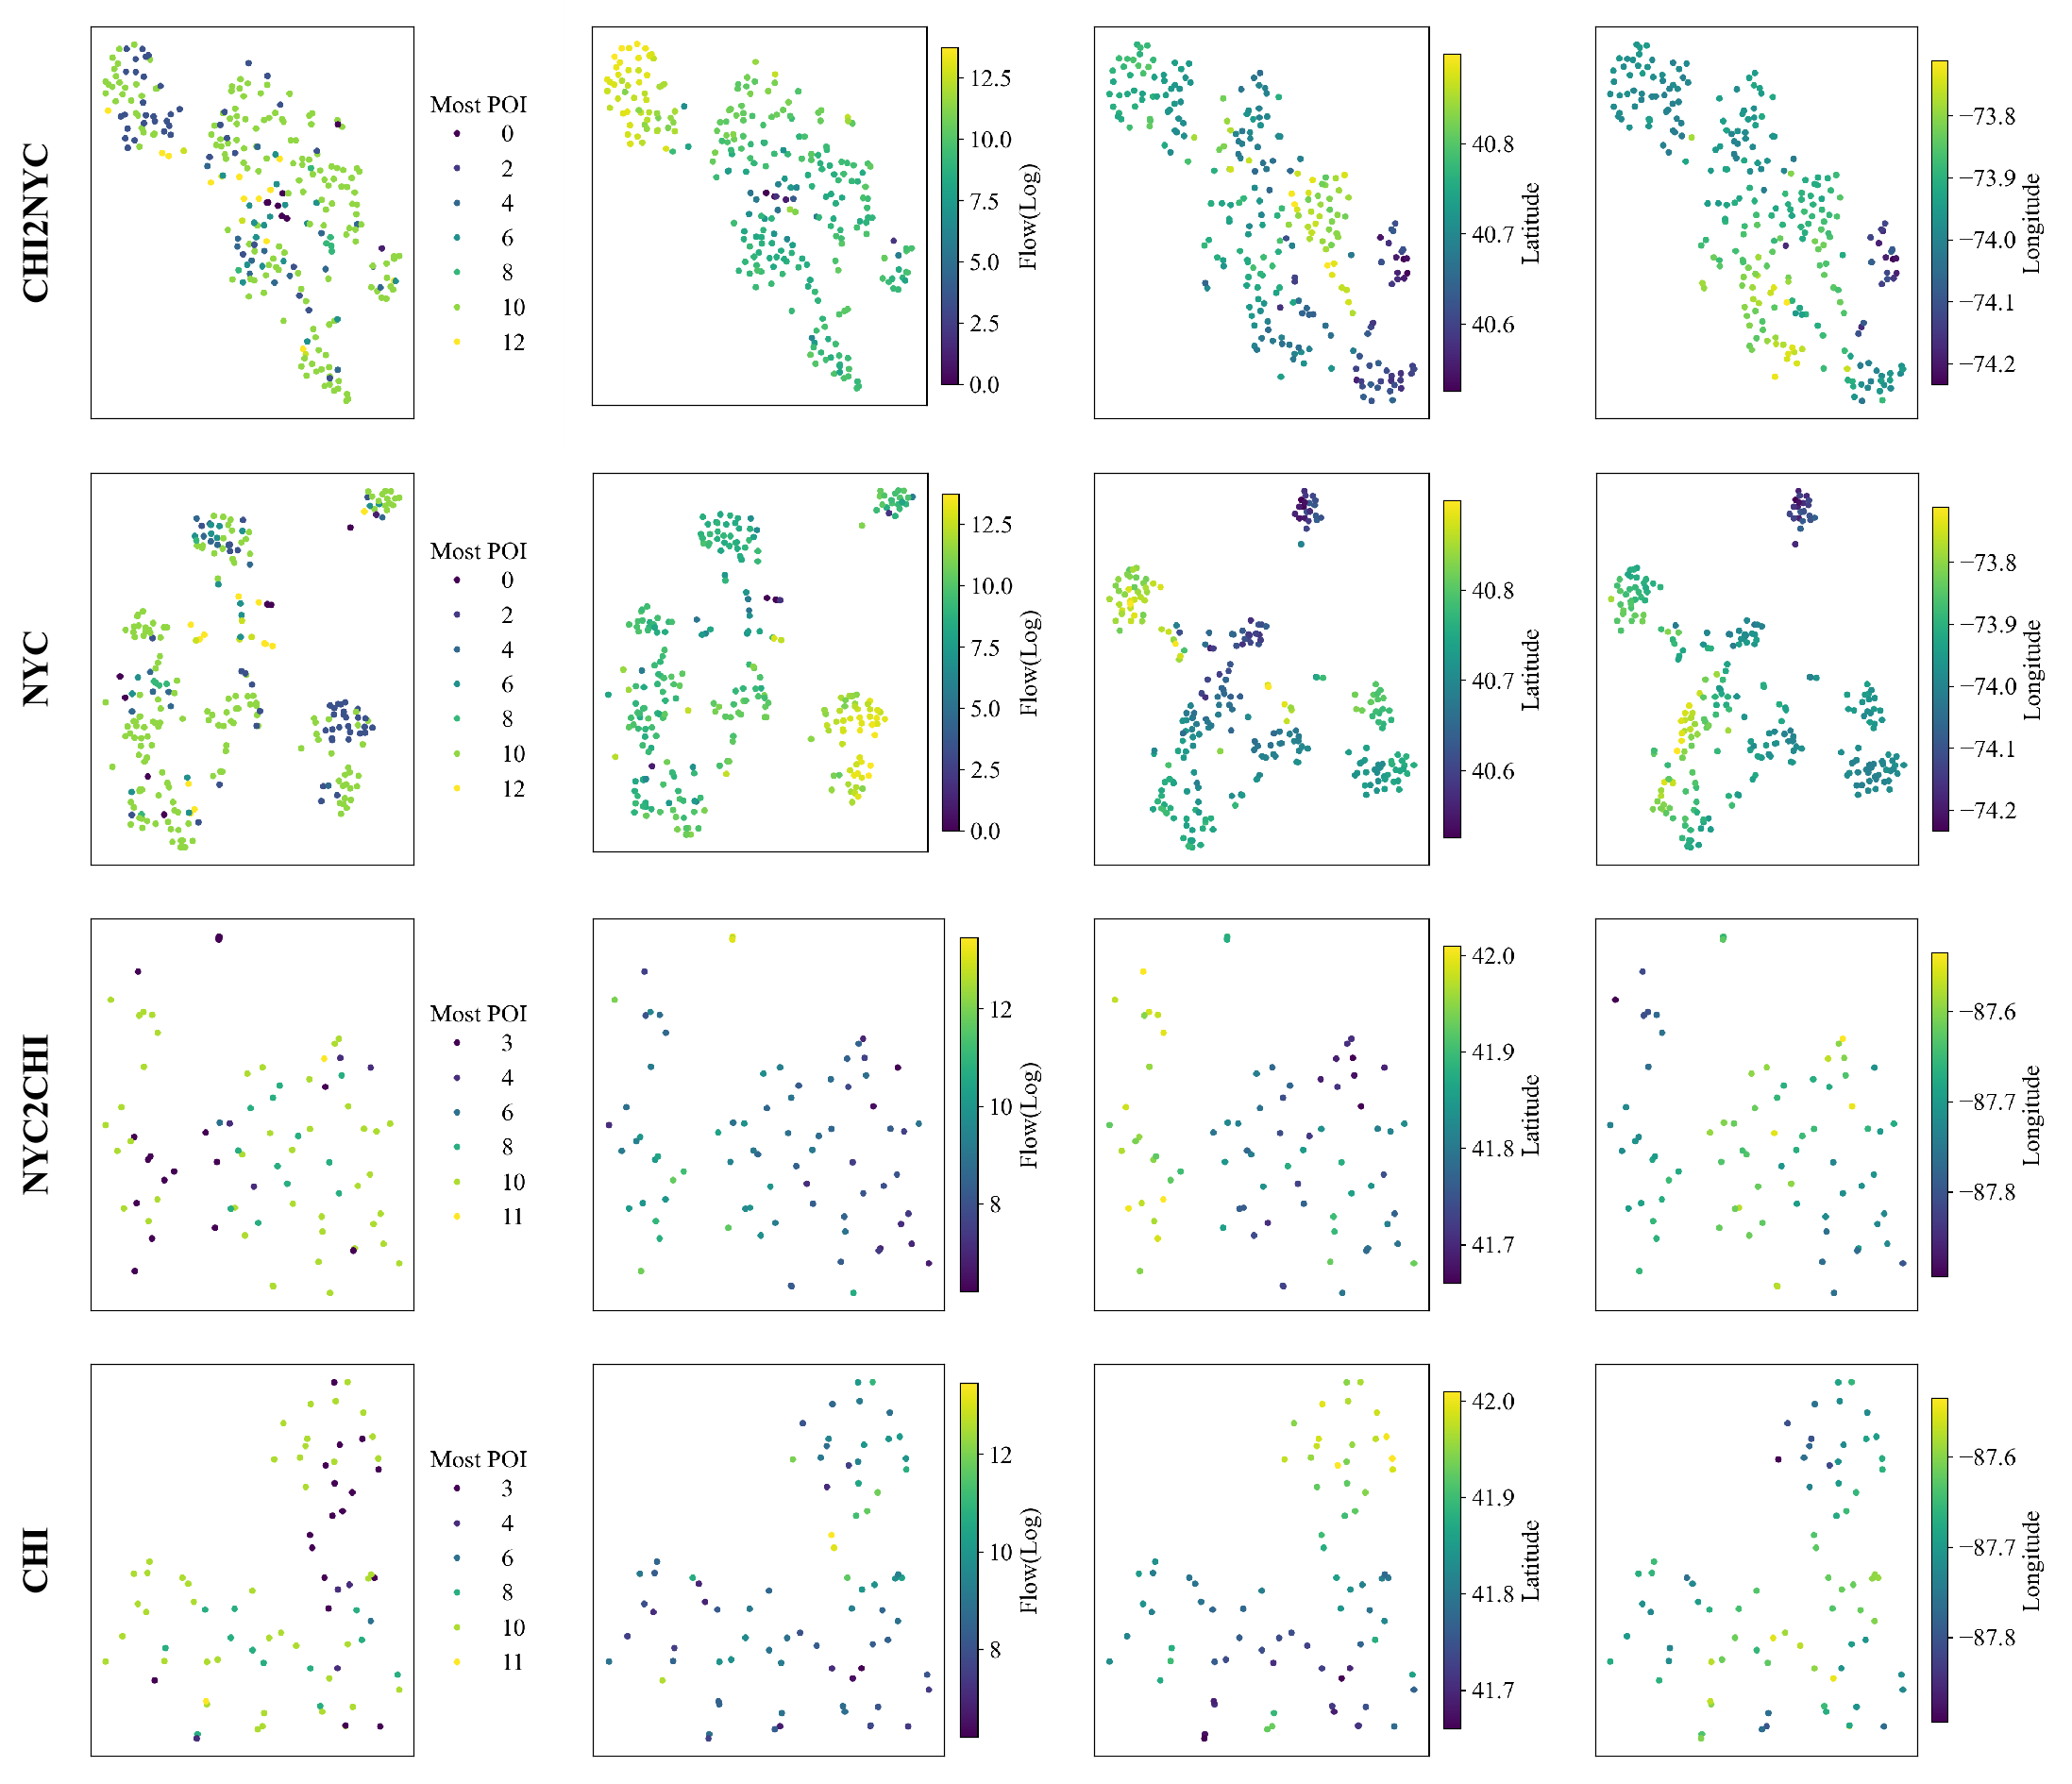
\includegraphics[width=0.99\textwidth]{fig/visualization_v2.png} % Reduce the figure size so that it is slightly narrower than the column.
% 
\caption{Representation Visualization Results in both single-city and cross-city settings}
\label{fig:vr}
\end{figure*}

% 在本章节中，我们对我们的实验设置和可视化结果做出进一步阐释。我们的代码可以在该链接中获取。
In this section, we further explain our experimental setup and visualization results. Our code is available at this link\footnote{https://anonymous.4open.science/r/MAP-STAR-HZX5213}.

\subsection{Datasets}
% 我们的实验主要在New York City(NYC)和Chicago(CHI)两个城市进行。为了在预训练阶段构建heterogeneous subgraph，我们分别收集了两个城市的区域划分、POI和交通流量数据。其中区域划分我们分别采用了NYC TLC\footnote{https://www.nyc.gov/site/tlc\label{fn:tlc}} and CHI Data Portal Community Areas\footnote{https://data.cityofchicago.org\label{fn:CDP}}的划分方式，分别将NYC和CHI分为275个和77个互不重合的网格。POI我们基于OpenStreetMap (OSM)\footnote{https://www.openstreetmap.org/}的数据进行统计。该数据包含POI点的名称（NAME）、类别（CATEGORY）、子类别（SUBCATEGORY）和经纬度（LON, LAT）字段。我们分别基于New York州和Illinois州的数据利用经纬度字段将这些POI点映射到区域中，为每个区域生成一个 $\text{max}_{\text{cate}}$ 维度的一维向量，向量中每个元素代表该区域包含该类别POI的数量。最后将区域间该向量的余弦相似度作为区域之间的POI相似度。此外我们从NYC TLC\footref{fn:tlc}和CHI Data Portal Community Areas\footref{fn:CDP}收集两个城市的出租车记录用于构建人口流动数据。我们收集了从2024.01.01-2024.06.30的出租车乘车记录，将乘车数据聚合为以小时为单位的inflow数据和OD数据as shown in Table \ref{tab:data_statistics}.最终我们基于这三个数据构建heterogeneous subgraphs $\mathcal{G}_i^{\text{sub}}$。

Our experiments are conducted on two major U.S. cities—New York City (NYC) and Chicago (CHI).
During pre-training, we construct heterogeneous subgraphs using three data sources for each city: administrative regions, points of interest (POIs), and taxi mobility records.
\begin{itemize}
    \item \textbf{Administrative regions.} For NYC we adopt the NYC TLC partition\footnote{https://www.nyc.gov/site/tlc\label{fn:tlc}}, and for CHI we use the Community Areas provided by the Chicago Data Portal\footnote{https://data.cityofchicago.org\label{fn:CDP}}. This yields 275 non-overlapping zones in NYC and 77 in CHI.
    \item \textbf{Points of interest.} POIs are extracted from OpenStreetMap (OSM)\footnote{https://www.openstreetmap.org/}. Each POI record contains (NAME, CATEGORY, LON, LAT). Using the coordinates, we assign POIs located in New York State and Illinois State to their corresponding regions, and aggregate them into a $\text{max}_{\text{cate}}$-dimensional vector for every region; each element counts the POIs of a specific category. Cosine similarity between these vectors defines the POI-based similarity between any pair of regions.
    \item \textbf{Taxi mobility.} Taxi trip records are taken from NYC TLC\footref{fn:tlc} and the Chicago Data Portal\footref{fn:CDP}. We collect rides from 2024-01-01 to 2024-06-30 and aggregate them into hourly inflow matrices and origin–destination (OD) matrices (see Table~\ref{tab:data_statistics}).
\end{itemize}
\begin{table}[!htbp]
\centering
    {
        \begin{tabular}{c|ccc}
        \hline
        City     & \#Nodes & \#Time Step    & \#Time Span\\ \hline
        NYC      & 275   & 4368  & 2024.1.1-2024.6.30   \\
        CHI      & 77    & 4368  & 2024.1.1-2024.6.30   \\
        \hline
        \end{tabular}
    }
    \caption{Statistics of pretrain datasets.}
    \label{tab:data_statistics}
\end{table}
Finally, the three data sources are integrated to construct the heterogeneous subgraphs $\mathcal{G}_i^{\text{sub}}$ used throughout this study.

% 为了验证上游预训练表征能够捕获丰富的区域语义信息，并用于各项Urban Computing的任务中，我们从NYC Open Data\footnote{https://opendata.cityofnewyork.us/data/} 和 CHI Data Portal\footref{fn:CDP}中收集了crime和crash两个下游任务的数据。此外我们还基于NPP-VIIRS-like NTL data \cite{DVN/YGIVCD_2020}的数据收集了nightlight下游任务的数据。具体来说，我们筛选了发生在from 2024-01-01 to 2024-06-30时间内的crime和crash，分别在NYC和CHI筛选得到了超过129000条和125000条的crime记录与超过42000条和54000条的crash记录，并基于记录中事件发生的经纬度将这些记录聚合到region中。而NPP-VIIRS-like NTL data按照1km*1km的grid记录了全球nightlight数据，我们基于grid的中心点筛选在每个区域内的网格计算平均nightlight作为该网格的nightlight预测数据。最终构建形成三个下游任务数据。
To evaluate whether the upstream pre-training representations capture rich regional semantics that generalize to diverse Urban Computing tasks, we curate three downstream datasets, crime, crash, and night-light.
\begin{itemize}
    \item \textbf{Crime and crash.} Incident reports are obtained from NYC Open Data\footnote{https://opendata.cityofnewyork.us/data/} and the Chicago Data Portal\footref{fn:CDP}. We select all records that occurred between 2024-01-01 and 2024-06-30, yielding more than 129{,}000 crime events and 42{,}000 traffic crashes in NYC, and over 125{,}000 crime events and 54{,}000 crashes in CHI. Each record is geocoded to latitude–longitude coordinates and then aggregated to its corresponding region.
    \item \textbf{Night-light.} We extract nocturnal luminosity from the NPP-VIIRS-like NTL dataset~\cite{DVN/YGIVCD_2020}, which reports global night-light intensity on a 1,km × 1,km grid. For every region, we average the intensities of all grid cells whose centroids fall within the region boundary, producing the regional night-light target. 
\end{itemize}
% These procedures result in three downstream datasets used to assess the semantic quality of cross-city region embeddings.



\subsection{Baselines}

We compare MAP-STAR with nine state-of-the-art baselines drawn from three methodological groups and evaluate them under two experimental protocols. In the single-city scenario, MAP-STAR is assessed against classical graph-based region representation methods. In the cross-city scenario, we additionally benchmark MAP-STAR against sequence-based and region transfer learning approaches.

\noindent\textbf{Graph-based Region Representation Learning}
\begin{itemize}
\item \textbf{HREP}\cite{HREP}: learns universal region embeddings by constructing heterogeneous relations and prompt-based downstream objectives.
\item \textbf{ReCP}\cite{ReCP}: fuses multi-view data via intra-view contrastive learning plus reconstruction, and inter-view contrastive prediction.
\item \textbf{ST-ReP}~\cite{ST-ReP}: designs multi-scale flow reconstruction and flow-prediction losses to obtain transferable region representations.
\end{itemize}

\noindent\textbf{Sequence-based Methods}
\begin{itemize}
\item \textbf{PatchTST}\cite{PatchTST}: encodes mobility series into patch sequences and exploits a Transformer encoder to model patch-level dependencies.
\item \textbf{TSLANet}\cite{TSLANet}: employs a lightweight CNN-based adaptive network and Fourier transforms to capture temporal and frequency features.
\item \textbf{TimesURL}~\cite{TimesURL}: applies frequency–temporal data augmentation and instance-level contrastive learning for robust flow representations.
\end{itemize}



\noindent\textbf{Region Transfer Learning}
\begin{itemize}
\item \textbf{TransGTR}\cite{TransGTR}: introduces a structure generator that minimizes spatial feature discrepancies between source and target cities.
\item \textbf{CrossST}\cite{CrossST}: builds a Spatial–Temporal Pattern Bank on the source city to transfer the learned urban knowledge.
\item \textbf{CoRE}~\cite{CoRE}: aligns representation manifolds of two cities to transfer mobility knowledge.
\end{itemize}




\subsection{Experimental Implementations}
During pre-training, the input sequence is divided into patches of length 2016 using a sliding window of 168. OD matrices are calculated for the corresponding intervals to facilitate heterogeneous subgraph sampling. For each region node we sample its second-order neighborhood, selecting five first-order and five second-order neighbours to preserve a balanced local topology. For downstream evaluation, we compute the mean inflow for each region and the associated average OD matrix, which are then fed into the encoder. All experiments use a representation dimension of 128. Both pre-training and evaluation rely on the Adam optimiser with a fixed learning rate of 0.001. Early stopping is employed—with a patience of 30 epochs during pre-training and 50 epochs during evaluation—to ensure stable convergence and reliable performance estimates.

\subsection{Representation Visualization}
% 为了进一步探究MAP-STAR获取的区域表征的质量，我们分别利用在NYC和CHI两个源城市上预训练得到的模型，在single-city和cross-city两个setting上获取模型表征。之后为了可视化该表征是否有从三个视角采样的子图上学习城市有关的知识，我们将表征进行降维，分别以区域most poi, flow, latitude和longitu为label进行表征可视化如图 \ref{fig:vr}。表征可视化结果显示，不同label的表征在降维后形成不同的簇，从中可以看出MAP-STAR能够将区域间的POI相似信息、人口流量特征和地理临近性编码进入pattern-bank中，证明我们预训练表征的有效性。此外，不同的模型在相同城市上编码形成的表征分布具有相似性。例如NYC和CHI2NYC两行中，在利用longitude作为label进行可视化时，我们同样得到紫色的较为离群的簇，这验证了我们模型跨城市迁移的能力。
% To further examine the quality of the representations learned by MAP-STAR, we first pre-train the model on the two source cities, NYC and CHI, and obtain embeddings under both the single-city and cross-city settings. We then project these embeddings into a two-dimensional space and visualize them using four region-level labels, most frequent POI category, population flow, latitude, and longitude. The visualizations are presented in Fig.~\ref{fig:vr}.

% After dimensionality reduction, embeddings with different labels form clearly separated clusters. This indicates that MAP-STAR successfully encodes POI similarity, mobility patterns, and geographic proximity into the pattern bank, confirming the effectiveness of our pre-training strategy. Moreover, the embedding distributions produced by different models on the same target city exhibit similar structures. For instance, in the rows “NYC” and “CHI2NYC,” embeddings coloured by longitude both reveal an outlying purple cluster, demonstrating the model’s ability to transfer knowledge across cities.

To further examine the quality of the representations learned by MAP-STAR, we visualize region embeddings obtained under both single-city and cross-city settings. Specifically, MAP-STAR is pre-trained on NYC and CHI, and embeddings are extracted from models trained on NYC alone as well as models transferred from CHI to NYC. These embeddings are projected into a two-dimensional space using dimensionality reduction techniques for qualitative analysis.

To assess whether heterogeneous subgraph sampling enables the model to capture urban semantics from multiple complementary views, we visualize the embeddings using four region-level labels: most frequent POI category, population flow intensity, latitude, and longitude, as shown in Fig.~\ref{fig:vr}. After dimensionality reduction, embeddings associated with different labels form clearly separated clusters. This clustering pattern indicates that MAP-STAR effectively encodes functional similarity, mobility dynamics, and geographic proximity into a shared representation space.

Moreover, embedding distributions under different training settings exhibit highly consistent structures on the same target city. For example, in both “NYC” and “CHI2NYC” settings, longitude-colored visualizations reveal a similar outlying cluster, corresponding to geographically extreme regions. The preservation of such spatial structures across settings suggests that MAP-STAR learns transferable region representations that remain robust under cross-city distribution shifts.




% Uncomment only when your track requires the checklist inside the PDF.
% \input{ReproducibilityChecklist.tex}

\end{document}
